% =====================================================================
%  DOCUMENT COMPLET ET AUTONOME — a coller tel quel dans main.tex
%
%  Mode d'emploi Overleaf
%  ----------------------
%  1. Coller TOUT ce fichier dans main.tex (il commence par \documentclass
%     et se termine par \end{document}).
%  2. Televerser le dossier  figures/  a la racine du projet, avec les
%     six PDF : fig_pipeline, fig_architecture_reseau, fig_gains,
%     fig_courbe_420474, fig_courbe_170214, fig_courbe_393604.
%  3. Compiler en pdfLaTeX.
%
%  Paquets requis : graphicx, booktabs, amsmath, geometry.
%  Tous font partie de la distribution de base : rien a installer.
%  Les nombres sont ecrits a la main avec \, comme separateur de milliers :
%  pas de dependance a siunitx, qui est la cause d'erreur la plus frequente.
% =====================================================================

\documentclass[11pt,a4paper]{article}

\usepackage[utf8]{inputenc}
\usepackage[T1]{fontenc}
\usepackage[margin=2.5cm]{geometry}

\usepackage{graphicx}
\usepackage{booktabs}
\usepackage{amsmath}

\graphicspath{{figures/}{./}}

\setlength{\tabcolsep}{6pt}
\renewcommand{\arraystretch}{1.15}

\title{Émulation de courbes de charge résidentielles\\ et gisement de flexibilité}
\author{}
\date{}

\begin{document}
\maketitle

% =====================================================================
\section{Architecture des modèles}

La reconstitution d'une courbe de charge est séparée en deux questions de natures
différentes. \emph{Combien} un logement consomme dans l'année se prédit à partir de ses
seules caractéristiques statiques : c'est le rôle du modèle annuel. \emph{Comment} cette
consommation se répartit heure par heure demande la météo et les usages : c'est le rôle du
réseau récurrent, qui reçoit le niveau annuel en entrée plutôt que de le redécouvrir.

\begin{figure}[htbp]
  \centering
  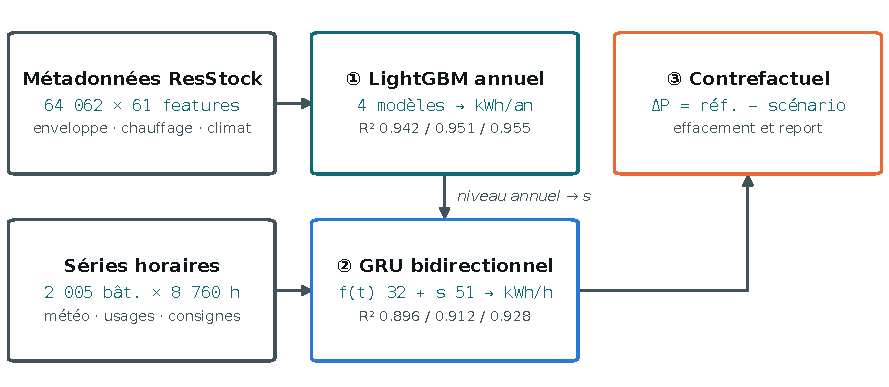
\includegraphics[width=\textwidth]{fig_pipeline.pdf}
  \caption{Chaîne de modélisation. Le modèle annuel fournit au réseau horaire le niveau de
  consommation de chaque usage ; le réseau horaire fournit à l'étude de flexibilité une
  courbe de charge sensible à la consigne de thermostat.}
  \label{fig:pipeline}
\end{figure}

\subsection{Réseau horaire}

Le réseau lit une semaine complète de conditions (168 pas horaires) et rend la consommation
de chacune de ces heures pour quatre usages. Il est \emph{non causal} : à l'heure $t$ il
accède à toute la semaine, passé et futur. Ce choix est légitime pour un émulateur de
simulation sur une année météo connue d'avance, et ne le serait pas en prévision temps réel.
Aucune consommation passée n'entre en entrée, ce qui permet d'appliquer le modèle à un
bâtiment jamais mesuré.

\begin{figure}[htbp]
  \centering
  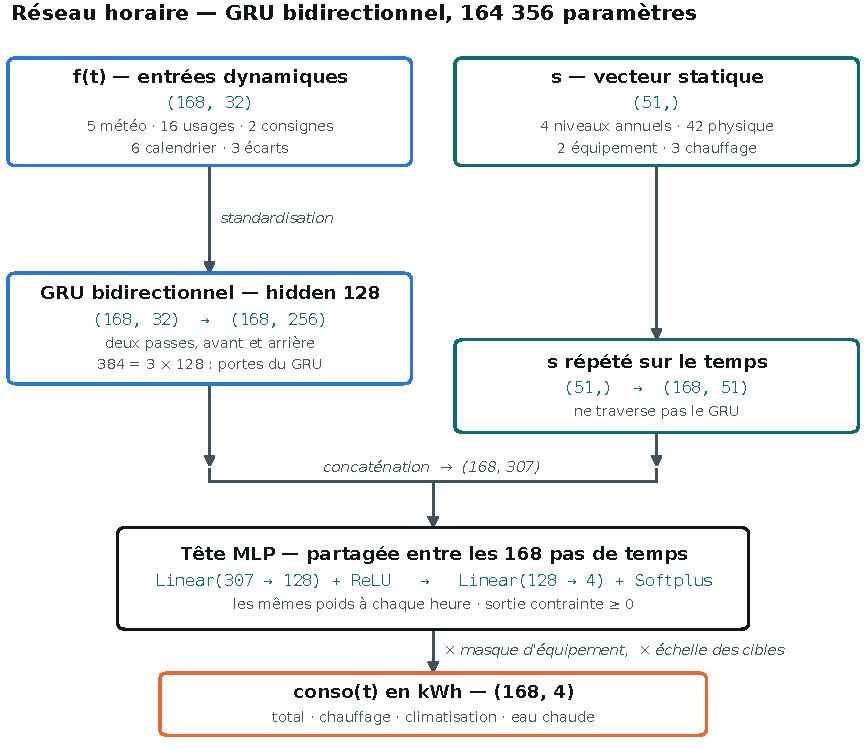
\includegraphics[width=0.92\textwidth]{fig_architecture_reseau.pdf}
  \caption{Architecture du réseau horaire. Les entrées dynamiques $f(t)$ traversent un GRU
  bidirectionnel ; le vecteur statique $s$ est concaténé à chaque pas de temps avant une
  tête MLP partagée. Le masque de sortie force à zéro les usages dont l'équipement est
  absent du logement.}
  \label{fig:architecture}
\end{figure}

Le besoin électrique de chauffage, troisième colonne dérivée de $f(t)$, traduit la chute du
rendement d'une pompe à chaleur avec le froid :
%
\begin{equation}
  \mathrm{COP}(t) = \min\!\Big(\mathrm{COP}_{b},\;
  \max\!\big(1,\; \mathrm{COP}_{b} \times (0{,}6 + 0{,}02\,T_{\mathrm{ext}}(t))\big)\Big),
  \qquad
  P_{\mathrm{elec}}(t) = \frac{\Delta\theta_{\mathrm{ch}}(t)}{\mathrm{COP}(t)},
  \label{eq:cop}
\end{equation}
%
où $\Delta\theta_{\mathrm{ch}}(t) = \max\big(0,\; \theta_{\mathrm{consigne}}(t) -
T_{\mathrm{ext}}(t)\big)$ est l'écart rectifié à la consigne, et
$\mathrm{COP}_{b} = \mathrm{HSPF}/3{,}412$ pour une pompe à chaleur, $1$ pour une
résistance électrique.

\begin{table}[htbp]
  \centering
  \caption{Dimensions et budget de paramètres du réseau horaire.}
  \label{tab:parametres}
  \begin{tabular}{llrr}
    \toprule
    Bloc & Tenseur & Forme & Paramètres \\
    \midrule
    GRU sens avant   & \texttt{weight\_ih}         & $(384, 32)$  & 12\,288 \\
                     & \texttt{weight\_hh} + biais & $(384, 128)$ & 49\,920 \\
    GRU sens arrière & \texttt{weight\_ih}         & $(384, 32)$  & 12\,288 \\
                     & \texttt{weight\_hh} + biais & $(384, 128)$ & 49\,920 \\
    Tête, couche 1   & \texttt{head.0}             & $(128, 307)$ & 39\,424 \\
    Tête, sortie     & \texttt{head.2}             & $(4, 128)$   & 516     \\
    \midrule
    \textbf{Total}   &                             &              & \textbf{164\,356} \\
    \bottomrule
  \end{tabular}
\end{table}

\begin{table}[htbp]
  \centering
  \caption{Composition des entrées du réseau horaire.}
  \label{tab:entrees}
  \begin{tabular}{llrl}
    \toprule
    & Groupe & Colonnes & Contenu \\
    \midrule
    \multicolumn{4}{l}{\textit{Entrees dynamiques f(t) — 32 colonnes}} \\
      & Météo               & 5  & température, humidité, vent, solaire direct et diffus \\
      & Usages horaires     & 16 & occupants, éclairage, électroménager, eau chaude \\
      & Consignes           & 2  & chauffage et climatisation (reconstruites) \\
      & Calendrier cyclique & 6  & sinus et cosinus de l'heure, du jour, du mois \\
      & Écarts dérivés      & 3  & écart chauffage, écart clim, besoin électrique \\
    \midrule
    \multicolumn{4}{l}{\textit{Vecteur statique s — 51 colonnes}} \\
      & Niveaux annuels      & 4  & prédictions du modèle annuel, hors échantillon \\
      & Physique             & 42 & agrégats d'enveloppe, constante de temps, ResStock \\
      & Présence équipement  & 2  & climatisation, chauffe-eau électrique \\
      & Système de chauffage & 3  & pompe à chaleur, COP saisonnier, mini-split \\
    \bottomrule
  \end{tabular}
\end{table}

\clearpage

% =====================================================================
\section{Résultats}

\subsection{Vue d'ensemble}

\begin{figure}[htbp]
  \centering
  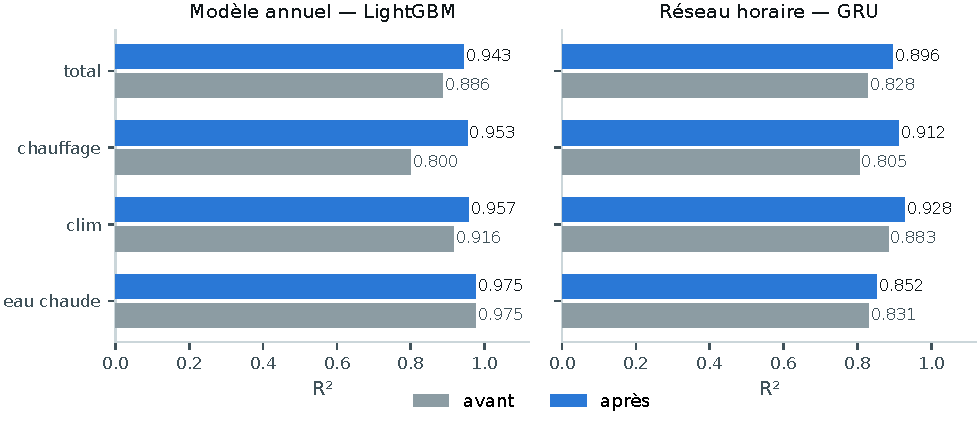
\includegraphics[width=\textwidth]{fig_gains.pdf}
  \caption{Coefficient de détermination par usage, avant et après l'ajout des variables de
  système de chauffage et de climat, la correction de la procédure de validation et
  l'élargissement du parc d'entraînement. Modèle annuel évalué sur 12\,813 logements de
  test, réseau horaire sur 101 bâtiments jamais vus.}
  \label{fig:gains}
\end{figure}

\begin{table}[htbp]
  \centering
  \caption{Performance du modèle annuel sur le jeu de test (12\,813 logements).
  RMSE en kWh/an.}
  \label{tab:lgbm}
  \begin{tabular}{lrrrrr}
    \toprule
    Usage & $R^2$ initial & $R^2$ final & $\Delta$ & RMSE finale & RMSE initiale \\
    \midrule
    Total         & 0,886 & 0,943 & $+0{,}057$ & 2\,377 & 3\,350 \\
    Chauffage     & 0,800 & 0,953 & $+0{,}153$ & 1\,649 & 3\,410 \\
    Climatisation & 0,916 & 0,957 & $+0{,}041$ & 645    & 902    \\
    Eau chaude    & 0,975 & 0,975 & $+0{,}000$ & 241    & 243    \\
    \bottomrule
  \end{tabular}
\end{table}

\begin{table}[htbp]
  \centering
  \caption{Performance du réseau horaire sur 101 bâtiments de validation. Le NMBE et le
  CV(RMSE) sont calculés par bâtiment puis médianés, selon l'ASHRAE Guideline 14 dont les
  critères au pas horaire sont $|\mathrm{NMBE}| \leq 10\,\%$ et
  $\mathrm{CV(RMSE)} \leq 30\,\%$.}
  \label{tab:reseau}
  \begin{tabular}{lrrrrr}
    \toprule
    Usage & $R^2$ initial & $R^2$ final & $\Delta$ & $|$NMBE$|$ médian & CV(RMSE) médian \\
    \midrule
    Total         & 0,828 & 0,896 & $+0{,}068$ & 8,3\,\%  & 24,3\,\% \\
    Chauffage     & 0,805 & 0,912 & $+0{,}107$ & 15,5\,\% & 59,1\,\% \\
    Climatisation & 0,883 & 0,928 & $+0{,}046$ & 12,1\,\% & 33,7\,\% \\
    Eau chaude    & 0,831 & 0,852 & $+0{,}021$ & 5,7\,\%  & 58,7\,\% \\
    \bottomrule
  \end{tabular}
\end{table}

Le $R^2$ est calculé sur l'ensemble des heures confondues et se trouve dominé par les gros
consommateurs ; il masque le biais de niveau. Le NMBE mesure ce biais, c'est-à-dire si le
modèle place la bonne quantité d'énergie sur l'année, tandis que le CV(RMSE) mesure la
dispersion, c'est-à-dire si les pics tombent au bon moment. Sur ces critères, seul le total
franchit le seuil de dispersion : le modèle place correctement l'énergie sur l'année sans
reproduire encore chaque pic de chauffage.

\subsection{Courbes reconstituées}

Les trois bâtiments présentés couvrent des situations opposées et sont choisis par climat
et par qualité de prédiction, non au hasard. Chaque figure superpose trois niveaux de
lecture pour une semaine de janvier et une semaine de juillet : la consommation totale, puis
l'usage dominant de la saison — chauffage en hiver, climatisation en été — et enfin la
température extérieure, qui explique la forme des deux courbes précédentes. La bande colorée
entre les deux tracés matérialise l'écart instantané : teintée du côté du modèle lorsqu'il
surestime, du côté de la simulation lorsqu'il sous-estime. Chaque panneau annonce ses cumuls
hebdomadaires, l'écart relatif correspondant et le coefficient de détermination de la
semaine.

\begin{figure}[htbp]
  \centering
  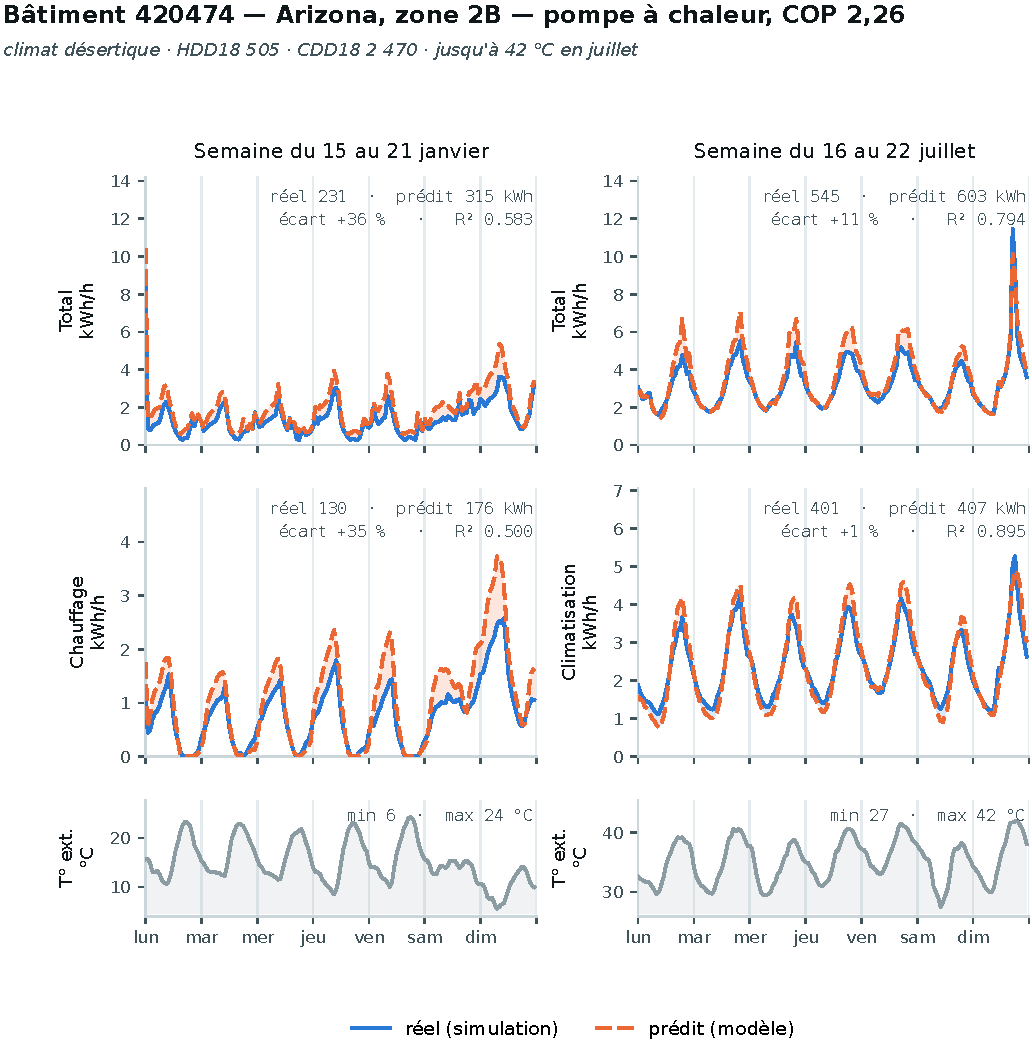
\includegraphics[width=\textwidth]{fig_courbe_420474.pdf}
  \caption{Bâtiment en climat désertique, équipé d'une pompe à chaleur. La climatisation
  domine largement le bilan et sa forme journalière est reproduite fidèlement, malgré des
  pointes légèrement surestimées.}
  \label{fig:courbe-az}
\end{figure}

\begin{figure}[htbp]
  \centering
  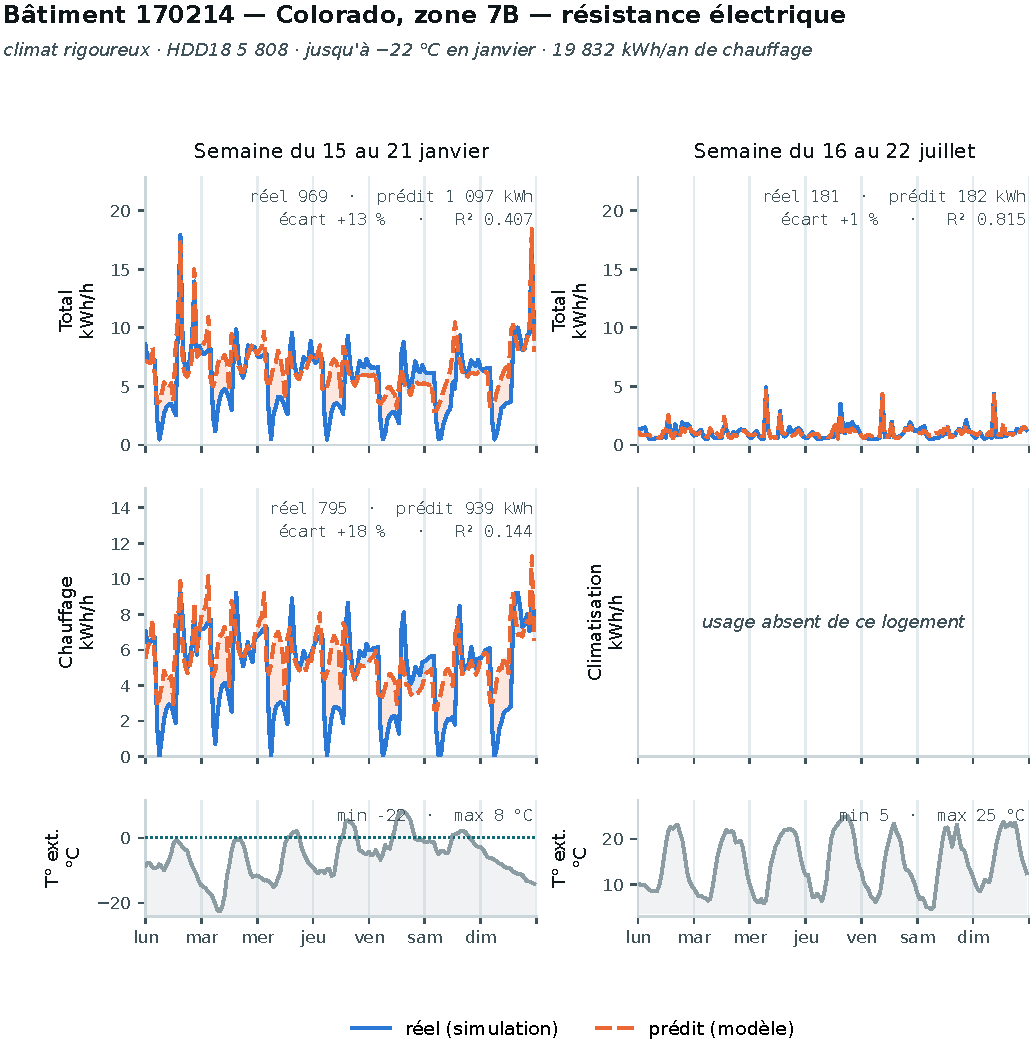
\includegraphics[width=\textwidth]{fig_courbe_170214.pdf}
  \caption{Bâtiment en climat rigoureux, chauffé par résistance électrique, avec des
  températures descendant à $-22\,^{\circ}$C. Le modèle suit correctement le niveau
  hebdomadaire mais lisse les creux profonds de la consommation réelle, ce qui explique un
  coefficient de détermination modeste malgré un écart de cumul limité. Ce logement ne
  possède pas de climatisation : le masque de sortie du réseau force cet usage à zéro.}
  \label{fig:courbe-co7b}
\end{figure}

\begin{figure}[htbp]
  \centering
  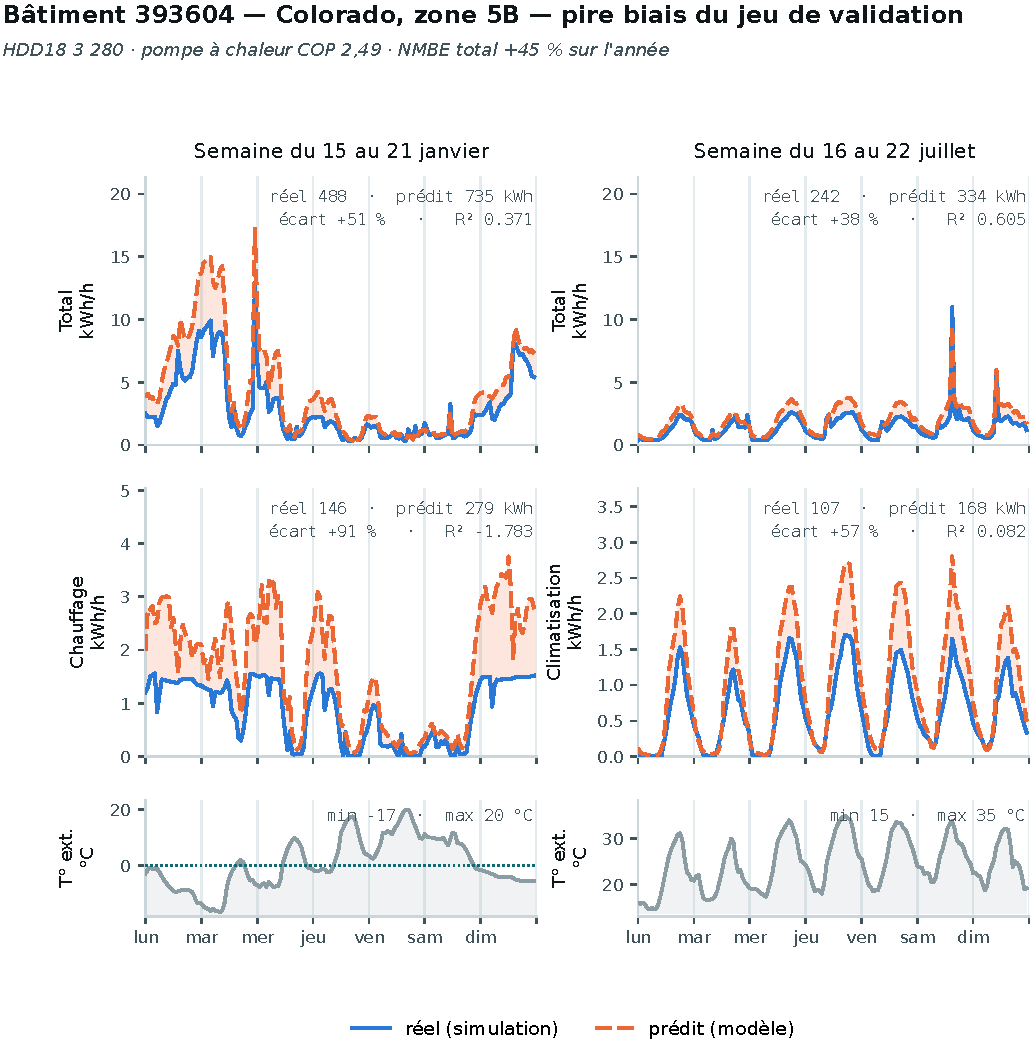
\includegraphics[width=\textwidth]{fig_courbe_393604.pdf}
  \caption{Bâtiment présentant le plus fort biais du jeu de validation. Le mode de
  défaillance y est visible directement : la forme journalière reste plausible, mais le
  niveau du chauffage est surestimé de près d'un facteur deux, y compris pendant les phases
  où la consommation réelle est stable. Le coefficient de détermination hebdomadaire du
  chauffage devient négatif, c'est-à-dire moins bon que la prédiction constante par la
  moyenne.}
  \label{fig:courbe-co5b}
\end{figure}

\begin{table}[htbp]
  \centering
  \caption{Bilans hebdomadaires des trois bâtiments illustrés, consommation totale en kWh.}
  \label{tab:bilans}
  \begin{tabular}{llrrrr}
    \toprule
    Bâtiment & Caractéristiques
      & \multicolumn{2}{c}{Semaine de janvier} & \multicolumn{2}{c}{Semaine de juillet} \\
    \cmidrule(lr){3-4} \cmidrule(lr){5-6}
      & & Réel & Prédit & Réel & Prédit \\
    \midrule
    420\,474 & Arizona, zone 2B, pompe à chaleur  & 231 & 315    & 545 & 603 \\
    170\,214 & Colorado, zone 7B, résistance      & 969 & 1\,097 & 181 & 182 \\
    393\,604 & Colorado, zone 5B, pompe à chaleur & 488 & 735    & 242 & 334 \\
    \bottomrule
  \end{tabular}
\end{table}

Ces trois cas illustrent le diagnostic porté par les indicateurs du tableau~\ref{tab:reseau} :
la structure temporelle est correctement apprise — alternance jour et nuit, réponse aux
vagues de froid, arrêt complet de la climatisation en hiver — tandis que l'erreur résiduelle
porte principalement sur le niveau de chauffage de certains bâtiments.

\clearpage

\subsection{Pistes écartées}

\begin{table}[htbp]
  \centering
  \caption{Variantes évaluées séparément, à parc, graine et jeu de validation constants.
  L'écart est donné sur le $R^2$ total, sauf mention contraire.}
  \label{tab:ecartees}
  \begin{tabular}{llr}
    \toprule
    Variante & Modèle & Écart \\
    \midrule
    Tête multiplicative (forme $\times$ niveau annuel)    & réseau & $-0{,}027$ (chauffage) \\
    Modulation FiLM du vecteur statique                   & réseau & $-0{,}008$ \\
    GRU à deux couches avec dropout                       & réseau & $-0{,}009$ \\
    Perte de Huber et réduction du pas sur plateau        & réseau & $-0{,}002$ \\
    Moyennes glissantes de température (24 et 72 h)       & réseau & $-0{,}007$ \\
    Apports solaires (surface équivalente $\times$ GHI)   & réseau & $-0{,}008$ \\
    Fenêtres glissantes au pas de 24 h                    & réseau & $+0{,}000$ \\
    Produit enveloppe $\times$ écart de température       & réseau & $+0{,}002$ \\
    Variables climatiques dans le vecteur statique        & réseau & $+0{,}008$ \\
    Transformation logarithmique de la cible              & annuel & $-0{,}015$ (chauffage) \\
    Objectif tweedie appliqué à l'eau chaude              & annuel & $-0{,}003$ \\
    \bottomrule
  \end{tabular}
\end{table}

Deux enseignements de méthode ressortent de ces essais. D'une part, ajouter de la structure
au modèle ne remplace pas une information manquante : la tête multiplicative encodait une
loi physique exacte et a pourtant dégradé les résultats, parce qu'elle déplaçait la
difficulté vers une grandeur absente du vecteur statique. D'autre part, le levier dominant
s'est révélé être le nombre de bâtiments d'entraînement et non l'architecture. À
configuration identique, passer de 503 à 2\,005 bâtiments apporte davantage que toutes les
variantes d'architecture réunies, qui sont toutes négatives. Le contraste avec les fenêtres
glissantes est net : sept fois plus de fenêtres sur les mêmes bâtiments n'apporte rien,
quatre fois plus de bâtiments apporte l'essentiel.

\end{document}
